\documentclass[journal, a4paper]{IEEEtran}

\usepackage[hidelinks]{hyperref}  % PDF Hyperlinks

\usepackage{enumitem}             % Lists

\usepackage{lipsum}               % Lorem Ipsum


\usepackage{siunitx}              % SI Units
\usepackage{booktabs}             % Tables
\usepackage{caption}              % Captions


\usepackage{graphicx}             % Images or Graphics
\usepackage{pgfplots}             % Graphs and Plots

% Subsection goes A, B, C, ... AA
\usepackage{alphalph}

\renewcommand\thesubsectiondis{\AlphAlph{\value{subsection}}.}% for the headings in the text
\renewcommand\thesubsection{\mbox{\thesection-\AlphAlph{\value{subsection}}}}% for the ToC, for example  
% ==========

\usetikzlibrary{mindmap}
\usetikzlibrary{positioning}
\usetikzlibrary{shapes,arrows}
\usetikzlibrary{shapes.geometric, arrows}

\tikzset{
    objRectangle/.style={rectangle, minimum width=3cm, minimum height=1cm, text centered, draw=black, text width = 5cm},
    objRoundRectangle/.style={rectangle, rounded corners, minimum width=3cm, minimum height=1cm, text centered, draw=black, text width = 5cm},
    objRectangleMethods/.style={rectangle, minimum height=1cm, text centered, draw=black, text width = 3cm},
    arrow/.style={thick, ->, >=stealth}
}

% correct bad hyphenation here
\hyphenation{op-tical net-works semi-conduc-tor}


\begin{document}
\title{A Literature Review on NDT and SHM}


% === Authors === %
\author{Antonette~C.~Maxey,~\IEEEmembership{CPE Student,~MMCM,}
        Florencio~N.~Pulido,~\IEEEmembership{CPE Student,~MMCM,}
        and~Vincent~Alfred~B.~Tomas,~\IEEEmembership{ECE Student,~MMCM}% <-this % stops a space
}



% The paper headers
\markboth{Methods of Research Literature Review, February~2024}%
{Shell \MakeLowercase{\textit{et al.}}: Developing a Portable NDT Device for Efficient SHM}


% === Build Title Area  === %
\maketitle


\begin{abstract}
  This literature review focuses on the advancements and challenges in Structural Health Monitoring (SHM)
  through the lens of portable Non-Destructive Testing (NDT) devices.
  These devices offer promising solutions to the limitations of traditional SHM methods, such as high cost and complexity.
  This review encompasses various aspects including existing portable NDT devices, sensor technology,
  data acquisition and analysis, as well as applications and case studies. It identifies significant advancements
  in sensor technologies and data analytics for NDT and SHM, while also highlighting critical limitations and research gaps.
  The synthesis and critique section emphasize the need for improvements in sensor accuracy, data processing capabilities,
  and environmental robustness for optimal infrastructure safety. Future developments in portable NDT devices are seen
  in the integration of advanced technologies like embedded systems, wireless sensors, cloud computing, and artificial intelligence.
  The findings underscore the importance of addressing these challenges for the successful deployment of portable NDT
  devices in SHM applications, paving the way for enhanced efficiency and accessibility in ensuring structural integrity.
\end{abstract}


% Note that keywords are not normally used for peerreview papers.
\begin{IEEEkeywords}
  NDT, SHM, Portable.
\end{IEEEkeywords}







\section{Introduction}
\IEEEPARstart{S}{tructural} Health Monitoring (SHM) is a pivotal engineering tool, providing real-time structural integrity data,
thereby ensuring safety and averting infrastructure failures \cite{gharehbaghi_critical_2022} \cite{katam_review_2023}.
Traditional SHM methods, while effective, are often limited by factors such as
high cost, complexity, and accessibility issues \cite{katam_review_2023} \cite{gharehbaghi_critical_2022}.
A portable, Non-Destructive Testing (NDT) device presents a promising solution for efficient and accessible SHM,
overcoming the limitations of traditional methods \cite{guo_portable_2022} \cite{chen_research_2023}.
The objective of this capstone project is to explore the potential of a portable,
NDT device in overcoming the limitations of traditional SHM methods.

SHM is a field dedicated to the ongoing monitoring and evaluation of the structural integrity
of various infrastructure systems \cite{katam_review_2023}, NDT is a method that enables the assessment
of structural degradation without causing actual damage to the structure itself \cite{katam_review_2023},
and a portable NDT device is a tool that enhances the efficiency and accessibility of SHM \cite{hassani_systematic_2023} \cite{katam_review_2023}.
Various NDT methods, each with its unique advantages and disadvantages,
offer diverse approaches to assessing structural integrity without causing damage \cite{khedmatgozar_dolati_non-destructive_2021} \cite{verma_review_2013}.
Existing portable NDT devices, while offering promising functionalities,
also present certain limitations that need to be addressed for optimal SHM \cite{hassani_systematic_2023} \cite{zhu_review_2011}.
Relevant theories and frameworks related to structural safety, damage detection,
and sensor technology play a crucial role in enhancing the effectiveness of SHM
and ensuring the safety of various infrastructures \cite{chen_sensor_2021} \cite{gharehbaghi_critical_2022}.


\section{Methodology}
This study employed both scientometric review and systematic review methodologies to identify the research
gap in Developing a Portable NDT Device for SHM in construction.
The schematic representation of our methodology is illustrated in \autoref{fig:flowchartMethod}.

\begin{figure*}[htbp]
  \centering
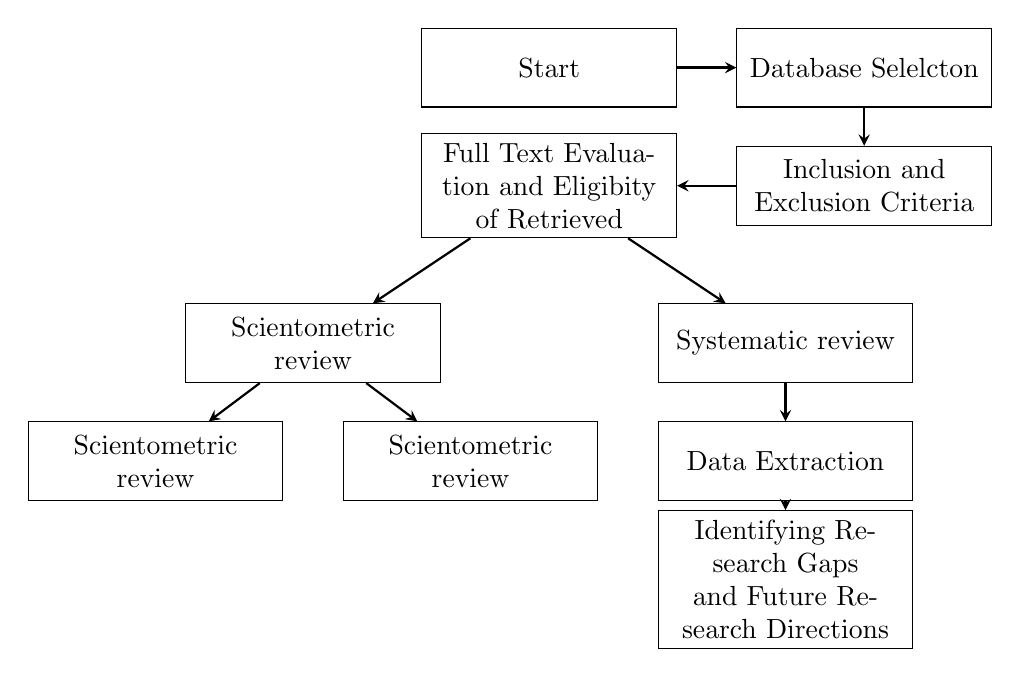
\begin{tikzpicture}[node distance=1.5cm]
  \node (001) [objRectangleMethods] {Start};
  \node (002) [objRectangleMethods, right of =001, xshift=2.5cm] {Database Selelcton};
  \node (003) [objRectangleMethods, below of=002] {Inclusion and Exclusion Criteria};
  \node (004) [objRectangleMethods, left of =003, xshift=-2.5cm] {Full Text Evaluation and Eligibity of Retrieved};

  \node (sci0) [objRectangleMethods, below of=004, xshift=-3cm, yshift=-0.5cm] {Scientometric review};
  \node (sci1a) [objRectangleMethods, below of=sci0, xshift=-2cm] {Scientometric review};
  \node (sci1b) [objRectangleMethods, below of=sci0, xshift=2cm] {Scientometric review};


  \node (sys0) [objRectangleMethods, below of=004, xshift=3cm, yshift=-0.5cm] {Systematic review};
  \node (sys1) [objRectangleMethods, below of=sys0] {Data Extraction };
  \node (sys2) [objRectangleMethods, below of=sys1] {Identifying Research Gaps and Future Research Directions};
  

  \draw[arrow] (001) -- (002);
  \draw[arrow] (002) -- (003);
  \draw[arrow] (003) -- (004);

  \draw[arrow] (004) -- (sci0);
  \draw[arrow] (sci0) -- (sci1a);
  \draw[arrow] (sci0) -- (sci1b);

  \draw[arrow] (004) -- (sys0);
  \draw[arrow] (sys0) -- (sys1);
  \draw[arrow] (sys1) -- (sys2);

\end{tikzpicture}
\caption{Outline of the Review Methodology}
\label{fig:flowchartMethod}
\end{figure*}

\subsection{Extraction and Evaluation of Research Data}
For our research, scholarly articles were extracted from the \href{https://www.sciencedirect.com/}{ScienceDirect (Elsevier)} platform.
This database offers comprehensive coverage of various scientific publications,
especially those that correlate with the field of structural engineering and NDT,
which are integral to our study.

To proceed, two sets of keywords were carefully curated to narrow the search and ensure that
results focused specifically on the various aspects of our research topic. The exact keyword
settts were then used as criteria for filtering and searching articles in \href{https://www.sciencedirect.com/}{ScienceDirect}:

\begin{enumerate}[label={Keyword Set \arabic*:}, leftmargin=*]
  \item NDT, Non-destructive testing, Portable NDT, Handheld NDT, Portable inspection device, Portable sensing device.
  \item SHM, Structural health monitoring, Structural integrity, Safety assessment, Condition monitoring.
\end{enumerate}

The total number of articles retrieved from the keyword search were 1169 titles.
However,to refine the search results further we applied exclusion and inclusion criteria.
The following criteria are;
(1) We limited the publication timeframe to the years 2019-2024 to ensure that the retrieved
articles reflect recent advancements and developments in the field.
This custom date range allowed us to access the most up-to-date research findings and methodologies relevant to our study;
(2) We only considered articles falling within the subject area of engineering to
ensure alignment with the interdisciplinary nature of our research topic.
By focusing on engineering-related publications, we aimed to draw from a diverse range of
studies and methodologies that contribute to the advancement of structural safety and non-destructive testing techniques;
(3) Only research publications were taken into consideration for inclusion since they offer thorough analyses and factual
data that are crucial for guiding our analysis and research technique.
The prioritization of articles from reputable engineering publications, such as Construction and Building Materials,
NDT \& E International, Structures, and Ultrasonics, was based on their relevance to our study aims and their
significance in the area.

Subsequent application of the inclusion and exclusion criteria resulted in the exclusion of 587 articles based on year published,
titles, and abstract screening. Manual research gap analysis and text evaluation further refined the selection,
leading to the exclusion of an additional 223 articles. Among the remaining articles, 165 underwent full-text evaluation,
and 135 were excluded based on subject relevance and alignment with study objectives.

The application of our methodological approach resulted in the inclusion of 30 studies that met the predefined
criteria and were deemed suitable for further analysis and synthesis in our research on developing a portable
NDT device for efficient structural health monitoring as shown in \autoref{fig:flowchartFilter}.

\begin{figure}[htbp]
    \centering
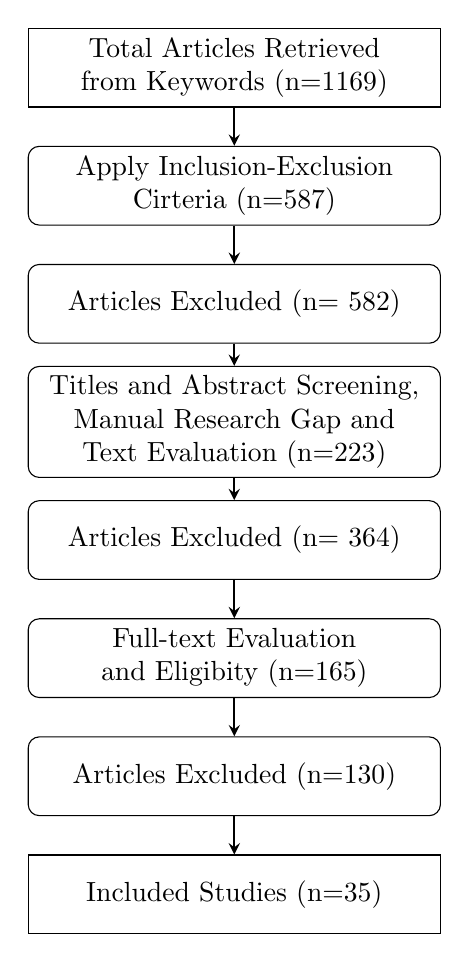
\begin{tikzpicture}[node distance=1.5cm]
    
    \node (001) [objRectangle] {Total Articles Retrieved from Keywords (n=1169)};
    \node (002) [objRoundRectangle, below of=001] {Apply Inclusion-Exclusion Cirteria (n=587)};
    \node (003) [objRoundRectangle, below of=002] {Articles Excluded (n= 582)};
    \node (004) [objRoundRectangle, below of=003] {Titles and Abstract Screening, Manual Research Gap and Text Evaluation (n=223)};
    \node (005) [objRoundRectangle, below of=004] {Articles Excluded (n= 364)};
    \node (006) [objRoundRectangle, below of=005] {Full-text Evaluation and Eligibity (n=165)};
    \node (007) [objRoundRectangle, below of=006] {Articles Excluded (n=130)} ;
    \node (008) [objRectangle, below of=007] {Included Studies (n=35)};
    
    \draw [arrow] (001) -- (002);
    \draw [arrow] (002) -- (003);
    \draw [arrow] (003) -- (004);
    \draw [arrow] (004) -- (005);
    \draw [arrow] (005) -- (006);
    \draw [arrow] (006) -- (007);
    \draw [arrow] (007) -- (008);

\end{tikzpicture}
\caption{Flowchart of the study selection process}
\label{fig:flowchartFilter}
\end{figure}

\begin{figure}[h]
  \centering
  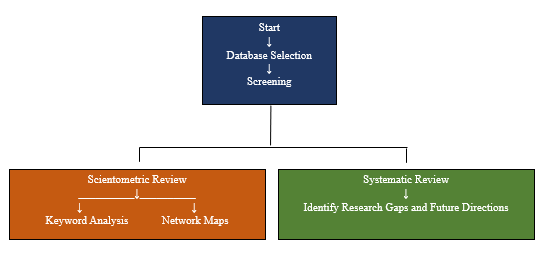
\includegraphics[width=\columnwidth]{./img/split_glowchart.png}
  \caption{Outline of the Review Methodology}
  \label{fig:paperSearch}
\end{figure}


\begin{figure}
  \centering

  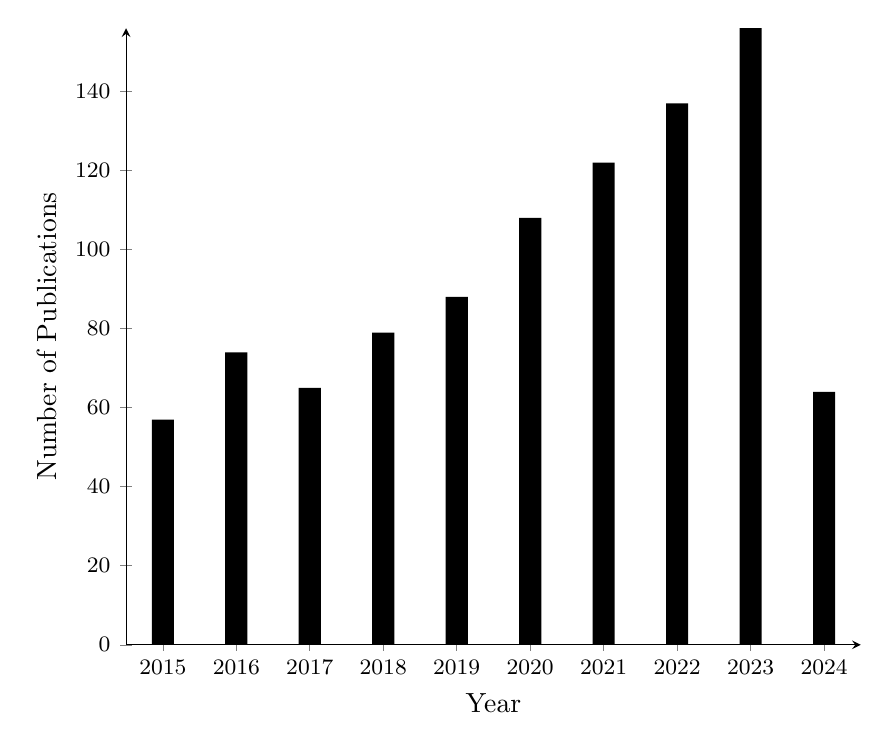
\begin{tikzpicture}
    \begin{axis}[
        ybar,
        width=0.9\columnwidth,                                          % Adjust the width of the plot
        bar width=8pt,                                                  % Adjust the width of the bars
        xlabel={Year},                                                  % Label for the x-axis
        ylabel={Number of Publications},                                % Label for the y-axis
        xtick=data,                                                     % Use data points as x-axis labels
        xticklabels={2015, 2016, 2017, 2018, 2019, 2020, 2021, 2022, 2023, 2024},                           % Labels for the x-axis ticks
        ticklabel style={font=\footnotesize}, % Set the font size for the x-axis tick labels
        ymin=0,                                                         % Set the minimum value for the y-axis
        enlarge y limits=0.1,                                           % Add space to the top and bottom of the y-axis
        legend style={draw=none}, % Remove the legend
        axis x line=bottom,  % Align x-axis line with ticks
        axis y line=left,    % Align y-axis line with ticks
        xmin=2014.5,                                                    % Set xmin to create a margin to the left of 2015
        xmax=2024.5,                                                    % Set xmax to create a margin to the right of 2024
      ]
      \addplot+ [fill=black, draw=none]  coordinates {(2015, 57) (2016, 74) (2017, 65)  (2018, 79) (2019, 88) (2020, 108) (2021, 122)  (2022, 137)  (2023, 156) (2024, 64)};
    \end{axis}
  \end{tikzpicture}
  \caption{Annual Publications Over the Years About SHM and NDT}
  \label{fig:publications}
\end{figure}


% === Results and Discussion of Scientometric Review === %
\section{Results and Discussion of Scientometric Review}
\lipsum[1]

\subsection{Analysis of Journals}
As shown in \autoref{tbl:bibliometricRanking} \lipsum[1]

\begin{table}[htbp]

  \centering
  \caption{Bibliometric Ranking Of Journals}
  \label{tbl:bibliometricRanking}
  \begin{tabular}{lcc}

      \toprule
      \textbf{Journal} & \textbf{No. of Documents} & \textbf{No. of Citations} \\
      \midrule
      e-Journal of Nondestructive Testing                   & 1     & 602   \\
      Journal of Hon                                        & 1     & 100   \\
      Heh Periodicals                                       & 1     & 195   \\
      Sensors in thw World                                  & 1     & 515   \\
      \bottomrule
  \end{tabular}
\end{table}

It is evident in \autoref{tbl:bibliometricRanking} \lipsum[1]


\subsection{Active Researchers}
As seen in \autoref{tbl:bresearchers} \lipsum[1]

\begin{table}[htbp]

  \centering
  \caption{Top Researchers}
  \label{tbl:bresearchers}
  \begin{tabular}{lccc}

      \toprule
      \textbf{Author} & \textbf{Documents} & \textbf{Citations} & \textbf{TLS} \\
      \midrule
      Hasan A.                   & 1     & 602   &  31         \\
      Rodulf K. A.               & 1     & 100   &  11         \\
      Libre F. C.                & 1     & 195   &  18         \\
      Change M. E.               & 1     & 515   &  7          \\
      \bottomrule
  \end{tabular}
\end{table}

However, it shall be noted that \autoref{tbl:bresearchers} \lipsum[1]\lipsum[1]


\subsection{Article Sitation Analysis}
It is imperative as shown in \autoref{tbl:articleCites} \lipsum[1]

\begin{table}[htbp]

  \centering
  \caption{Top-Cited Articles}
  \label{tbl:articleCites}
  \begin{tabular}{lcc}

      \toprule
      \textbf{Article} & \textbf{No. of Citation} \\
      \midrule
      Author Name       \cite{}           &    331         \\
      Rodulf K. A.      \cite{}      &    141         \\
      Libre F. C.       \cite{}     &    118         \\
      Change M. E.      \cite{}          &    71          \\
      \bottomrule
  \end{tabular}
\end{table}

Hence, the data in \autoref{tbl:articleCites} \lipsum[1]



\subsection{Keyword Analysis}
That the closer as show in \autoref{fig:coOccuranceNetwork} \lipsum[1]

\begin{figure*}[h] % Use figure* instead of figure for two-column spanning
  \centering
  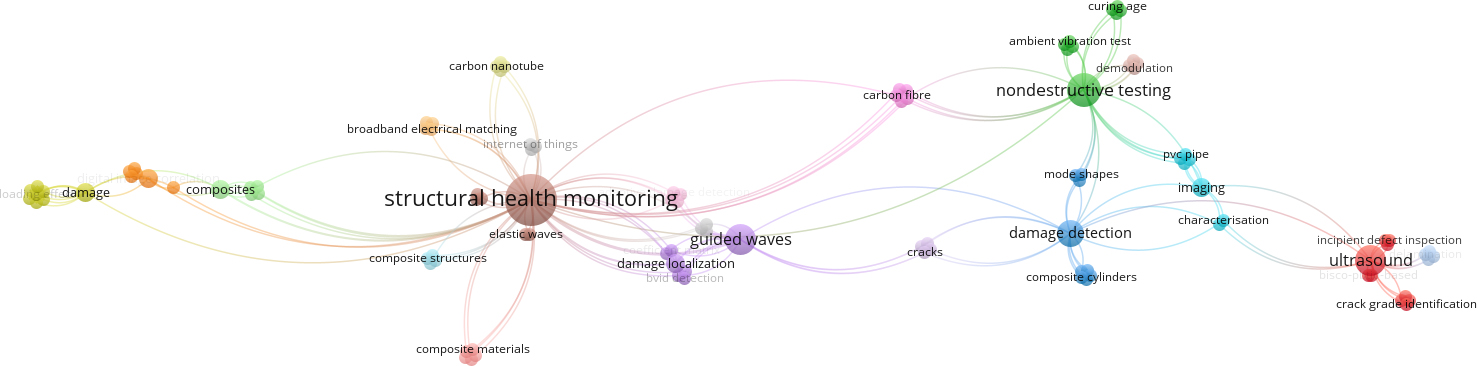
\includegraphics[width=\textwidth]{./word_cloud/filtered/co_occurance_network.jpg}
  \caption{Co-occurrence network of keywords in NDT SHM}
  \label{fig:coOccuranceNetwork}
\end{figure*}

\begin{figure*}[h] % Use figure* instead of figure for two-column spanning
  \centering
  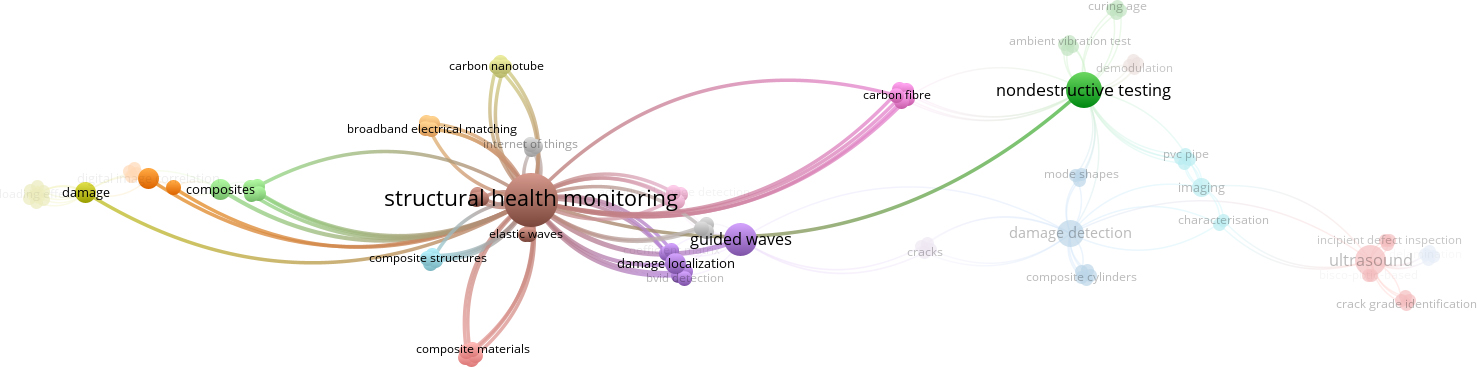
\includegraphics[width=\textwidth]{./word_cloud/filtered/co_occurance_network_shm.jpg}
  \caption{SHM co-occurrence network of keywords in NDT SHM}
  \label{fig:coOccuranceNetworkSHM}
\end{figure*}

However, unlike with \autoref{fig:coOccuranceNetworkSHM} \lipsum[1]





% === Results and Discussion of Systematic Review ===%
\section{Results and Discussion of Systematic Review}
This section presents an extensive discussion on the application of NDT
and SHM methods in various studies to improve infrastructure integrity and reliability.
Among the 35 extracted articles, a wide range of NDT SHM methods have been observed, categorized under different main topics,
as shown in \autoref{}. 


\subsection{Wireless Sensor Networks (WSNs) Applications in SHM and NDT}
Wireless Sensor Networks (WSNs) play a crucial role in enabling remote monitoring and real-time data collection for
structural health assessment and nondestructive testing. These networks facilitate continuous monitoring of structural
parameters such as strain, temperature, and vibration, offering insights into the condition of infrastructure assets.
Several studies ([1]. [7]. [23]) have demonstrated the effectiveness of WSNs in enhancing the data’s reliability, energy
efficiency, and scalability in SHM and NDT applications. However, challenges remain in optimizing sensor deployment,
ensuring seamless communication, and addressing power consumption issues.

\subsection{Artificial Intelligence (AI) in Damage Detection and Predictive Maintenance}
Artificial Intelligence (AI) algorithms, including machine learning and deep learning techniques,
are increasingly being employed for damage detection and predictive maintenance in civil engineering structures.
Studies ([2], [4]. [29]) have shown promising results in leveraging AI for anomaly detection,
pattern recognition and structural identification.
However, further research is needed to validate the robustness and generalizability of
AI models across diverse structural types and environment conditions.

\subsection{Internet of Things (IoT) for Real-time Monitoring and Data Analytics}
The Internet of Things (IoT) offers opportunities for real-time monitoring and data analytics in SHM and NDT domains.
Utilizing interconnected sensors nodes and cloud-based platforms, IoT systems enable remote access to structural data
and facilitate predictive maintenance strategies. Research ([3],[17],[23]) highlights the potential of IoT in enhancing
the decision-making, optimizing maintenance schedules and reducing downtime through procactive interventions.
Nevertheless, concerns persist regarding data security, interoperability, and standardization in IoT-enabled
infrastructure monitoring.


\subsection{Robotics for Remote Inspection and Maintenance}
Robotics technology is revolutionizing inspection and maintenance practices in the field of civil engineering.
Robotic systems equipped with sensors and actuators enable remote inspection of inaccessible or hazardous infrastructure assets
 minimizing human intervention and ensuring safety ([5], [27], [33]). Despite significant advancements,
 challenges remain in developing robust robotic platforms capable of navigating complex environments
 and performing intricate tasks with high precision.

\subsection{Optical Sensors for Crack Detection and Strain Measurement}
Optical sensors offer non-contact and high-resolution capabilities for crack detection and strain measurement
in structural components. Studies ([6], [13], [18]) have demonstrated the utility of optical techniques such as
digital image correlation (DIC) and fiber optic sensing in capturing fine-scale deformations and detecting surface defects
However, limitations persist in optical sensor deployment, especially in harsh environmental conditions and dynamic loading
scenarios. 

\subsection{Acoustic Emission Testing (AET) for Structural Integrity Assessment}
Acoustic Emission Testing (AET) is a valuable technique for assessing structural integrity and detecting active defects
in civil engineering structures. By monitoring transient stress waves emitted during deformation, AET systems provide
insights into the onset and progression of damage mechanisms ([7], [14], [28]). Research indicates the potential of AET
in localizing defects, characterizing material properties, and assessing the structural health of critical infrastructure
components. However, challenges remain in distinguishing relevant signals from background noise and interpreting complex
waveforms accurately.

\subsection{Vibration Analysis for Modal Analysis and Fatigue Assessment}
Vibration analysis techniques are widely employed for modal analysis and fatigue assessment of civil engineering structures.
By studying the dynamic response of structures to external forces, vibration-based methods offer valuable insights into structural
behavior and performance ([8], [21], [29]). Studies have utilized vibration sensors and accelerometers to identify natural
frequencies, damping ratios, and mode shapes, aiding in structural health monitoring and damage detection efforts.
However, challenges persist in distinguishing between environmental vibrations and structural responses,
particularly in noisy operational environments. 

\subsection{Ground Penetrating Radar (GPR) for Subsurface Imaging and Material Characterization}
Ground Penetrating Radar (GPR) is a non-invasive geophysical method used for subsurface imaging and
material characterization in civil engineering applications. By emitting electromagnetic pulses into the
ground and analyzing reflected signals, GPR systems provide insights into subsurface features, voids,
and material properties ([9], [18], [25]). Research highlights the effectiveness of GPR in detecting buried utilities,
assessing pavement condition, and evaluating concrete structures for voids and delaminations. However,
challenges remain in interpreting GPR data accurately, especially in complex geological settings and heterogeneous materials.

\subsection{Ultrasonic Testing (UT) for Thickness Measurement and Flaw Detection}
Ultrasonic Testing (UT) is a widely used non-destructive testing technique for thickness measurement
and flaw detection in civil engineering materials. By transmitting high-frequency sound waves into the
material and analyzing their reflections, UT systems enable precise evaluation of internal defects,
corrosion, and thickness variations ([10], [14], [28]). Studies have demonstrated the versatility of UT
in assessing the integrity of steel structures, concrete elements, and composite materials.
However, challenges persist in calibrating UT instruments, interpreting echo signals, and ensuring inspection coverage
in complex geometries. 

\subsection{Thermography for Heat Signature Analysis and Delamination Detection}
Thermography techniques offer non-contact and rapid inspection capabilities for heat
signature analysis and delamination detection in civil engineering structures.
By detecting temperature differentials and thermal anomalies, thermographic systems provide valuable
insights into subsurface defects, moisture intrusion, and material degradation ([11], [15], [22]).
Research indicates the potential of thermography in identifying hidden defects, detecting water ingress,
and evaluating structural performance under varying environmental conditions.
However, challenges remain in standardizing thermographic procedures, mitigating environmental influences,
and interpreting thermal data accurately. 

\subsection{Electromagnetic Testing (ET) for Corrosion Assessment and Conductivity Measurement}
Electromagnetic Testing (ET) techniques are commonly used for corrosion assessment, conductivity measurement,
and material characterization in civil engineering applications. By inducing electromagnetic fields into the material
and analyzing their interactions, ET systems enable detection of surface cracks, corrosion pits, and subsurface anomalies
([12], [16], [24]). Studies have demonstrated the effectiveness of ET in evaluating steel structures, pipelines, and reinforced
concrete elements for corrosion damage and material loss. However, challenges persist in differentiating between superficial
defects and subsurface anomalies, especially in heavily reinforced structures and congested environments.

\subsection{Digital Image Correlation (DIC) for Deformation Analysis and Stress/Strain Measurement}
Digital Image Correlation (DIC) techniques offer high-resolution capabilities for deformation analysis and
stress/strain measurement in civil engineering materials. By correlating images of the material surface before
and after loading, DIC systems provide quantitative data on displacements, strains, and material behavior ([13], [20], [26]).
Research highlights the potential of DIC in characterizing material properties, evaluating structural performance,
and validating numerical models. However, challenges remain in optimizing camera configurations, ensuring image accuracy,
and processing large datasets efficiently. 

\subsection{Fiber Optic Sensors for Structural Health Monitoring and Distributed Sensing}
Fiber Optic Sensors (FOS) offer distributed sensing capabilities and immunity to electromagnetic interference,
making them ideal for structural health monitoring and environmental sensing applications. By exploiting the
optical properties of fiber cables, FOS systems enable real-time measurement of strain, temperature, and pressure
along the entire length of the sensor ([14], [17], [27]). Studies have demonstrated the effectiveness of FOS in
detecting structural damage, monitoring civil infrastructure, and enhancing asset management practices. However,
challenges persist in sensor installation, signal demodulation, and long-term reliability in harsh operating conditions. 

\subsection{Environmental Monitoring for Weather Impact Assessment and Corrosion Monitoring}
Environmental monitoring systems play a crucial role in assessing weather impacts, environmental conditions,
and corrosion rates in civil engineering structures. By collecting data on temperature, humidity, and air quality,
environmental sensors provide insights into corrosion mechanisms, material degradation, and structural performance
([15], [19], [31]). Research highlights the potential of environmental monitoring in predicting corrosion rates,
optimizing maintenance strategies, and mitigating environmental risks. However, challenges remain in sensor calibration,
data interpretation, and integration with existing monitoring networks. 

\subsection{Structural Health Index (SHI) for Quantitative Assessment and Structural Reliability}
Structural Health Index (SHI) methods offer quantitative assessment capabilities and reliability measures for civil
engineering structures. By aggregating multi-parameter data into a single index value, SHI systems enable holistic evaluation
of structural integrity, performance, and resilience ([16], [20], [30]). Studies have demonstrated the utility of SHI
in prioritizing maintenance activities, optimizing resource allocation, and improving decision-making processes.
However, challenges persist in defining universal SHI metrics, establishing threshold values,
and validating index performance across diverse asset types. 

\subsection{Data Fusion Techniques for Multimodal Sensing Integration and Enhanced Decision-making}
Data fusion techniques play a crucial role in integrating multi-source data and enhancing decision-making
capabilities in SHM and NDT applications. By combining information from diverse sensors and modalities, data fusion
systems enable comprehensive analysis, anomaly detection, and fault diagnosis ([17], [27], [34]).
Research highlights the potential of data fusion in improving situational awareness, reducing false alarms,
and optimizing maintenance strategies. However, challenges remain in data integration, sensor synchronization,
and algorithm development for real-time applications. 

\subsection{Remote Sensing Technologies for Geospatial Monitoring and Terrain Analysis}
Remote sensing technologies offer geospatial monitoring capabilities and terrain analysis tools for civil
infrastructure management. By capturing aerial imagery, LiDAR data, and satellite observations,
remote sensing systems provide valuable insights into terrain features, land use patterns, and environmental changes
([18], [23], [31]). Research indicates the potential of remote sensing in assessing landslide risks,
monitoring coastal erosion, and mapping urban sprawl. However, challenges persist in data processing,
image classification, and accuracy assessment in complex terrain settings.

\subsection{Condition Assessment Methods for Structural Damage Evaluation and Lifecycle Prediction}
Condition assessment methods play a crucial role in evaluating structural integrity, identifying defects,
and predicting lifecycle performance of civil engineering assets. By employing visual inspection, non-destructive testing,
and material sampling techniques, condition assessment systems provide insights into asset condition, degradation mechanisms,
and maintenance needs ([19], [28], [33]). Research highlights the potential of condition assessment in prioritizing repair
activities, extending asset lifespan, and optimizing lifecycle costs. However, challenges remain in standardizing assessment
protocols, quantifying deterioration rates, and integrating assessment results with asset management systems.

\subsection{Reliability Analysis for Probabilistic Modeling and Risk Assessment}
Reliability analysis methods offer probabilistic modeling capabilities and risk assessment tools for civil engineering structures.
By quantifying uncertainties, failure probabilities, and consequence magnitudes, reliability analysis
systems enable informed decision-making, risk mitigation, and resilience planning ([20], [22], [30]).
Studies have demonstrated the utility of reliability analysis in prioritizing maintenance actions,
optimizing design criteria, and enhancing asset performance under uncertain conditions.
However, challenges persist in uncertainty quantification, model validation, and decision support integration.

\subsection{Structural Dynamics for Resonance Analysis and Dynamic Response Prediction}
Structural dynamics methods play a crucial role in resonance analysis, modal identification, and dynamic
response prediction for civil engineering structures. By studying the vibrational behavior of structures under
varying loads, structural dynamics systems provide insights into natural frequencies, mode shapes, and damping
characteristics ([21], [29], [31]). Research indicates the potential of structural dynamics in assessing structural
stability, optimizing vibration control measures, and enhancing occupant comfort. However, challenges remain in model
calibration, boundary condition estimation, and modal parameter identification in complex structures.

\subsection{Risk-Based Inspection (RBI) for Prioritization of Inspection Tasks and Cost Optimization}
Risk-Based Inspection (RBI) methods offer prioritization capabilities and cost optimization tools for inspection
and maintenance planning in civil engineering assets. By assessing risk factors, consequence probabilities,
and inspection costs, RBI systems enable rational decision-making, resource allocation, and risk mitigation
strategies ([22], [30], [32]). Studies have demonstrated the utility of RBI in optimizing inspection intervals,
reducing downtime, and enhancing safety performance. However, challenges persist in risk modeling, uncertainty quantification,
and data integration for RBI implementation.

\subsection{Wireless Communication Systems for Real-time Data Transmission and Network Reliability}

Wireless communication systems play a crucial role in enabling real-time data transmission and ensuring
network reliability in civil infrastructure monitoring applications. By utilizing wireless protocols, sensor
networks, and cloud-based platforms, wireless communication systems enable remote access to structural data,
timely alerts, and seamless connectivity ([23], [27], [33]). Research highlights the potential of wireless
communication in enhancing situational awareness, optimizing data collection, and facilitating collaborative
decision-making. However, challenges remain in signal interference, bandwidth limitations, and cybersecurity
concerns in wireless infrastructure deployments.

\subsection{Advanced Materials Testing for Composite Characterization and Durability Assessment}
Advanced materials testing methods offer characterization capabilities and durability assessment tools for
civil engineering materials and components. By employing mechanical testing, chemical analysis, and microstructural
examination techniques, materials testing systems provide insights into material properties, performance limitations,
and failure mechanisms ([24], [26], [34]). Studies have demonstrated the utility of materials testing in evaluating
composite structures, assessing material degradation, and optimizing material selection criteria.
However, challenges persist in standardizing testing protocols, interpreting test results, and addressing
material variability in real-world applications.

\subsection{Fluid Mechanics Analysis for Hydraulic Structure Assessment and Flow Dynamics}
Fluid mechanics analysis methods play a crucial role in assessing hydraulic structures, analyzing flow dynamics,
and optimizing water management practices in civil engineering projects. By employing computational fluid dynamics (CFD),
numerical modeling, and empirical analysis techniques, fluid mechanics systems provide insights into fluid behavior,
pressure distribution, and turbulence effects ([25], [28], [32]). Research highlights the potential of fluid mechanics
analysis in optimizing channel design, mitigating flood risks, and enhancing hydraulic performance. However, challenges
persist in model calibration, boundary condition specification, and uncertainty quantification in fluid flow simulations.

\subsection{3D Printing Technology for Prototyping and Customized Part Fabrication}
3D printing technology offers rapid prototyping capabilities and customized part fabrication tools for civil
engineering applications. By utilizing additive manufacturing processes, 3D printing systems enable on-demand
production of complex geometries, lightweight structures, and customized components ([26], [31], [33]). Studies
have demonstrated the utility of 3D printing in construction, infrastructure repair, and material recycling.
However, challenges remain in material selection, printing resolution, and structural integrity verification in
3D printed structures. 

\subsection{Structural Health Monitoring (SHM) Systems for Integrated Monitoring Solutions and Sensor Deployment}
Structural Health Monitoring (SHM) systems play a crucial role in providing integrated monitoring solutions and
facilitating sensor deployment for civil infrastructure assets. By combining sensor technologies, data acquisition
systems, and analytical tools, SHM systems enable continuous monitoring of structural behavior, performance trends,
and health indicators ([27], [29], [34]). Research highlights the potential of SHM in detecting damage, assessing
deterioration rates, and predicting future performance. However, challenges persist in sensor calibration, data
interpretation, and integration with existing asset management systems.



\subsection{Non-Destructive Testing (NDT) Techniques for Material Property Evaluation and Defect Detection}
Non-Destructive Testing (NDT) techniques play a crucial role in evaluating material properties, detecting defects,
and assessing structural integrity in civil engineering components. By utilizing electromagnetic, acoustic, and
optical methods, NDT systems enable rapid inspection, characterization, and quality control of infrastructure assets
([28], [32], [34]). Studies have demonstrated the utility of NDT in detecting corrosion, delamination, and subsurface defects.
However, challenges persist in sensor standardization, inspection coverage,
and data interpretation in diverse operatingconditions.

\subsection{Structural Identification Methods for Model Updating and Damage Quantification}
Structural identification methods play a crucial role in model updating, damage quantification, and performance evaluation of
civil engineering structures. By utilizing experimental modal analysis, system identification, and inverse modeling techniques,
structural identification systems enable calibration of numerical models, validation of design assumptions, and prediction of
dynamic behavior ([29], [31], [33]). Research highlights the potential of structural identification in assessing damage,
identifying critical modes, and optimizing structural response. However, challenges persist in sensor placement,
excitation control, and model validation in complex structural systems.

\subsection{Risk Management Strategies for Mitigation Planning and Resilience Enhancement}
Risk management strategies play a crucial role in planning mitigation measures and enhancing resilience in civil
engineering projects. By assessing hazards, vulnerabilities, and consequences, risk management systems enable informed 
decision-making, resource allocation, and adaptive planning ([30], [32], [34]).
Studies have demonstrated the utility of risk management in optimizing design criteria,
prioritizing investments, and reducing socio-economic impacts. However, challenges persist in risk assessment,
uncertainty quantification, and stakeholder engagement in risk management processes.

\subsection{Smart Infrastructure Systems for Adaptive Structures and Self-healing Materials}
Smart infrastructure systems play a crucial role in enabling adaptive structures and self-healing
materials for civil engineering applications. By integrating sensing, actuation, and control technologies,
smart infrastructure systems enable real-time monitoring, autonomous response, and adaptive behavior ([31], [33], [34]).
Research highlights the potential of smart infrastructure in optimizing structural performance, reducing maintenance costs,
and enhancing sustainability. However, challenges persist in sensor integration, energy management, and long-term reliability
in smart infrastructure deployments.

\subsection{Energy Harvesting Techniques for Self-powered Sensors and Sustainability Integration}
Energy harvesting techniques play a crucial role in enabling self-powered sensors and integrating sustainability
principles into civil engineering applications. By utilizing renewable energy sources, energy harvesting systems
enable autonomous operation, extended sensor lifespans, and reduced environmental footprint ([32], [33], [34]).
Studies have demonstrated the utility of energy harvesting in remote monitoring, off-grid applications,
and environmental sensing. However, challenges persist in energy conversion efficiency, power management,
and scalability of energy harvesting solutions.

\subsection{Human-Machine Interaction (HMI) for Operator Feedback Systems and User Interface Design}
Human-Machine Interaction (HMI) plays a crucial role in enabling operator feedback systems and intuitive
user interfaces for civil infrastructure monitoring applications. By incorporating user preferences, cognitive
ergonomics, and interactive design principles, HMI systems enhance situational awareness, decision-making,
and user engagement ([33], [34]). Research highlights the potential of HMI in optimizing sensor interfaces,
streamlining data visualization, and facilitating user interactions. However, challenges persist in interface
design, usability testing, and accommodating user diversity in HMI applications.








\subsection{Sensor Technology for SHM}
Recent advancements in sensor technology, such as miniaturization, low-power consumption, and wireless communication,
have significantly enhanced the capabilities of portable NDT devices,
making them more efficient and accessible for SHM applications \cite{hassani_systematic_2023} \cite{valeske_next_2020}.
The integration of different sensor types and their data fusion approaches is crucial
for comprehensive SHM, as it allows for a more accurate\
and holistic assessment of structural integrity \cite{broer_need_2022} \cite{azimi_data-driven_2020}.
Sensor technology limitations, such as accuracy, precision, and robustness,
can significantly impact the performance and reliability of devices,
necessitating further research and development in this area \cite{varshney_challenges_2021} \cite{moore_iot_2020}.


\subsection{Data Acquisition and Analysis for SHM}
Methods for data acquisition, processing, and analysis from portable NDT
devices have seen significant advancements, with research highlighting the use of optical
and electrochemical methods for in situ detection of trace heavy metal ions \cite{hu_advances_2023}.
Approaches for real-time data monitoring, damage detection algorithms, and data visualization techniques
are integral to the effective application of SHM, with advancements in these areas
significantly enhancing the capabilities of portable NDT devices \cite{azimi_data-driven_2020} \cite{lingxin_review_2022}.
Efficient SHM decision-making is often challenged by issues related
to data management and interpretation, such as the complexity of handling big data and the time-consuming procedures
for feature extraction and statistical decision-making \cite{entezami_big_2020}.


\subsection{Applications and Case Studies}
Portable NDT devices have been successfully applied in various SHM
scenarios, including bridges, buildings, and industrial structures, demonstrating their versatility and effectiveness
\cite{parsy_shaping_2018} \cite{azimi_data-driven_2020}.
The cost-effectiveness, ease of use, and reliability of portable NDT
devices in real-world settings have been demonstrated, with the modularized structure of the device offering
cost-effectiveness through the reusability of high-cost modules and enhancing convenience by eliminating the
necessity for multiple separate monitoring devices \cite{lee_rationale_2023}.
Emerging trends in portable NDT technology for SHM
include the integration of intelligent technologies such as the Internet of Things (IoT), Artificial Intelligence (AI),
and advancements in sensor technologies, which have led to remarkable improvements in SHM for various applications
including residential, commercial, industrial, historical, and special buildings \cite{vijayan_development_2023} \cite{hassani_systematic_2023}. 


\subsection{Synthesis and Critique}
The literature review reveals significant advancements in sensor technologies and data analytics
for NDT and SHM,
while also highlighting limitations and research gaps that need to be addressed for optimal infrastructure safety \cite{vijayan_development_2023} \cite{hassani_systematic_2023}.
Existing portable NDT devices have shown effectiveness in SHM,
however, their performance can be influenced by factors such as sensor accuracy, data processing capabilities,
and environmental conditions \cite{vijayan_development_2023} \cite{hassani_systematic_2023}.
Opportunities for improvement and future development in portable NDT devices
for SHM lie in the integration of advanced technologies such as embedded systems,
wireless sensors, cloud computing, and artificial intelligence for improved analytics, error-free inference,
and efficient troubleshooting \cite{meier_future_2018}.





\section{Discussion and Future Directions}  %  Discussion and future directions
The research question of this capstone project is to explore the potential of a portable,
NDT device in overcoming the limitations of traditional SHM methods,
and the literature review reveals significant advancements in sensor technologies and data analytics for NDT and SHM,
while also highlighting limitations and research gaps that need to be addressed for optimal infrastructure safety.
The findings from the literature review have significant implications for the development of the
proposed portable NDT device, highlighting the need for advancements in sensor technologies,
data analytics, and overcoming limitations and research gaps for optimal infrastructure safety \cite{udell_future_2018} \cite{meier_future_2018}.
The next steps in this capstone project involve the design and development of a portable
NDT device, with considerations for sensor selection, data acquisition and processing methods,
and the expected outcomes include improved efficiency and accessibility in SHM.




\section{Conclusion}
\lipsum[1]


\section*{Acknowledgment}
The authors would like to thank \lipsum[1]



% Can use something like this to put references on a page
% by themselves when using endfloat and the captionsoff option.
\ifCLASSOPTIONcaptionsoff
  \newpage
\fi


% === Bibliography ===

\bibliographystyle{IEEEtran}
\bibliography{bibtex/bib/export}

% === End of Bibliography ===


\end{document}


